\scanpage{88}
\mspage{$\overline{\underline{\mathrm{VI}}}_{\mathrm B}$}
% A long oblique cancellation descends from beside VI B to the bottom of the sheet.
\deleted{Demander Raynaud détails \unsure{Abstracts|Abstraits|travaux} SGA 3}

\deleted{Prendre SGA 2 / Donner SGA 2}

\deleted{Prendre exemplaire vert SGA 1}

\deleted{Donner Demazure rabiot de Segal.}

\diagram{\begin{tikzcd}[ampersand replacement=\&,column sep=small,row sep=small]
X\arrow[r]\arrow[d,"f"']\& A\arrow[dl]\\
S\&
\end{tikzcd}}

\deleted{$D$ diviseur relatif sur $X$, \uline{strict\textsuperscript{t.}} \uline{alg. équiv. à} $0$ \deleted{sur chaque fibre} i.e définit une section de}
\diagram{\begin{tikzcd}[ampersand replacement=\&,row sep=small]
\deleted{\unsure{\underline{\operatorname{Pic}}^0_{A/S}|\underline{\operatorname{Pic}}_{X/S}}}\simeq\underline{\operatorname{Pic}}^{00}_{X/S}\\
A^*=\underline{\operatorname{Pic}}^0_{A/S}\arrow[u,"\unsure{\simeq|2}"']
\end{tikzcd}}
\diagram{\begin{tikzcd}[ampersand replacement=\&,column sep=small,row sep=small]
{\unsure{\cdot|0}}\arrow[r]\& V(R^1\underline O_{A^*})\arrow[r]\& E(A^*)\arrow[r]\& A^*\arrow[r]\&0\\
\&W({R^1\underline O_{A^*}}^\vee)\arrow[u,equal]\&\&\&\\
\&\omega_A\arrow[u,equal]\&\&\&
\end{tikzcd}}

\deleted{Par image inverse on trouve un fibré principal sous $\omega_A$, donc aussi sous $R^1f_*(\Omega^1_{X/S})$ $(\longleftarrow\omega_A)$. Interprétation ?}

\deleted{On considère}
\[
\deleted{\unsure{\Omega^1_{X/S}|\underline\Omega^1_{X/S}}(D)}\qquad
\deleted{\Omega^1_{X/S}\{D\}}\qquad \omega
\]
\figure{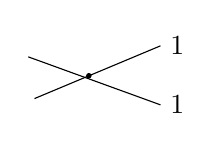
\begin{tikzpicture}[x=1cm,y=1cm]
\draw (0,0.05)--(1.6,.72) node[right] {$1$};
\draw (-.08,.58)--(1.6,-.03) node[right] {$1$};
\fill (.69,.34) circle (.035);
\end{tikzpicture}}
\[
f\omega=\varpi\qquad \omega=\frac{\varpi}{f}\qquad \widehat\omega=\frac{df}{f}
\]
\[
\operatorname{res}_{x}\omega\qquad \omega_i-\frac{df}{f}\qquad
\omega_i-\frac{df}{f}\quad\text{holomorphe au voisinage de}
\]
\[
\underline{\operatorname{Div}}_{X/S}\overset{\unsure{d\log f|d\log/S}}{\hookrightarrow}\underline R_{X/S}(\underline\Omega^1_{X/S})/\underline\Omega^1_{X/S}
\]
% The initial stroke curves upward at the left of the shaft.
% archive sheet number: 87
